%%%%%%%%%%%%%%%%%%%%%%%%%%%%%%%%%%%%%%%%%
% A beamer poster style for the ACET Conference 2022. 
% Written by Ye Kyaw Thu, Affiliate Professor, CADT, Cambodia
% Last updated: 28 June 2022
% email: yktnlp@gmail.com
%
% Based on the oxford-poster (https://github.com/gbaydin/oxford-poster)
% Based on the I6pd2 style created by Thomas Deselaers an Philippe Dreuw.
%
% Dreuw & Deselaer's Poster
% LaTeX Template
% Version 1.0 (11/04/13)
%
% Created by:
% Philippe Dreuw and Thomas Deselaers
% http://www-i6.informatik.rwth-aachen.de/~dreuw/latexbeamerposter.php
%
% This template has been downloaded from:
% http://www.LaTeXTemplates.com
%
% License:
% CC BY-NC-SA 3.0 (http://creativecommons.org/licenses/by-nc-sa/3.0/)
%
%%%%%%%%%%%%%%%%%%%%%%%%%%%%%%%%%%%%%%%%%

%----------------------------------------------------------------------------------------
%   PACKAGES AND OTHER DOCUMENT CONFIGURATIONS
%----------------------------------------------------------------------------------------

\documentclass[final,hyperref={pdfpagelabels=false}]{beamer}

\usepackage[orientation=landscape,size=a0,scale=1.3]{beamerposter} % Use the beamerposter package for laying out the poster with a portrait orientation and an a0 paper size

\usetheme{ACET}

\usepackage[utf8]{inputenc} % allow utf-8 input
\usepackage{blindtext}
\usepackage{amsmath,amsthm,amssymb,latexsym} % For including math equations, theorems, symbols, etc
\usepackage[document]{ragged2e}
\usepackage{times}\usefonttheme{professionalfonts}  % Uncomment to use Times as the main font
\usefonttheme[onlymath]{serif} % Uncomment to use a Serif font within math environments
%\boldmath % Use bold for everything within the math environment
\usepackage{booktabs} % Top and bottom rules for tables
\usepackage{microtype}

\usecaptiontemplate{\small\structure{\insertcaptionname~\insertcaptionnumber: }\insertcaption} % A fix for figure numbering

\newcommand{\shrink}{-15pt}

\def\imagetop#1{\vtop{\null\hbox{#1}}}

\let\oldbibliography\thebibliography
\renewcommand{\thebibliography}[1]{\oldbibliography{#1}
\setlength{\itemsep}{-10pt}}

%----------------------------------------------------------------------------------------
%   TITLE SECTION 
%----------------------------------------------------------------------------------------
\title{\Huge CADT Beamer Poster Template} % Poster title
\author{Author 1, Author 2, Author 3}
\institute{Department of Engineering Science, Cambodia Academy of Digital Technology\\\vspace{4mm}
\texttt{\{author1,author2,author3\}@cadt.edu.kh}}

%----------------------------------------------------------------------------------------
%   FOOTER TEXT
%----------------------------------------------------------------------------------------
\newcommand{\leftfoot}{} % Left footer text
\newcommand{\rightfoot}{} % Right footer text


%----------------------------------------------------------------------------------------

\begin{document}
\addtobeamertemplate{block end}{}{\vspace*{2ex}} % White space under blocks

\begin{frame}[t] % The whole poster is enclosed in one beamer frame

\begin{columns}[t] % The whole poster consists of three major columns, each of which can be subdivided further with another \begin{columns} block - the [t] argument aligns each column's content to the top

  \begin{column}{.02\textwidth}\end{column} % Empty spacer column

%%%%%%%%%%%%%%%%%%%%%%%%%%%%%%%%%%%%%%%%%%
%% Column 1
%%%%%%%%%%%%%%%%%%%%%%%%%%%%%%%%%%%%%%%%%%

  \begin{column}{.3\textwidth} % 1st column

    \vspace{\shrink}          
    \begin{block}{1. Introduction}
      \begin{itemize}
        \item {\bf Symbol Grounding $\times$ Chatting}
        \item Research on language acquisition and symbol grounding (focus on the acquisition of physically grounded knowledge through utterances that express physical things, such as objects and motions)
        \item Most of the previous studies have focused on learning without any prior symbolic knowledge
        \item The problem of how to acquire physically grounded knowledge based on grounded utterances through natural interaction has yet to be explored
        \item We focus on object-teaching utterances as grounded utterances
      \end{itemize}
    \end{block}

    \begin{block}{2. Experimental Environment}
      %Block text \cite{le-2016-inference-compilation}...
      \begin{center}
        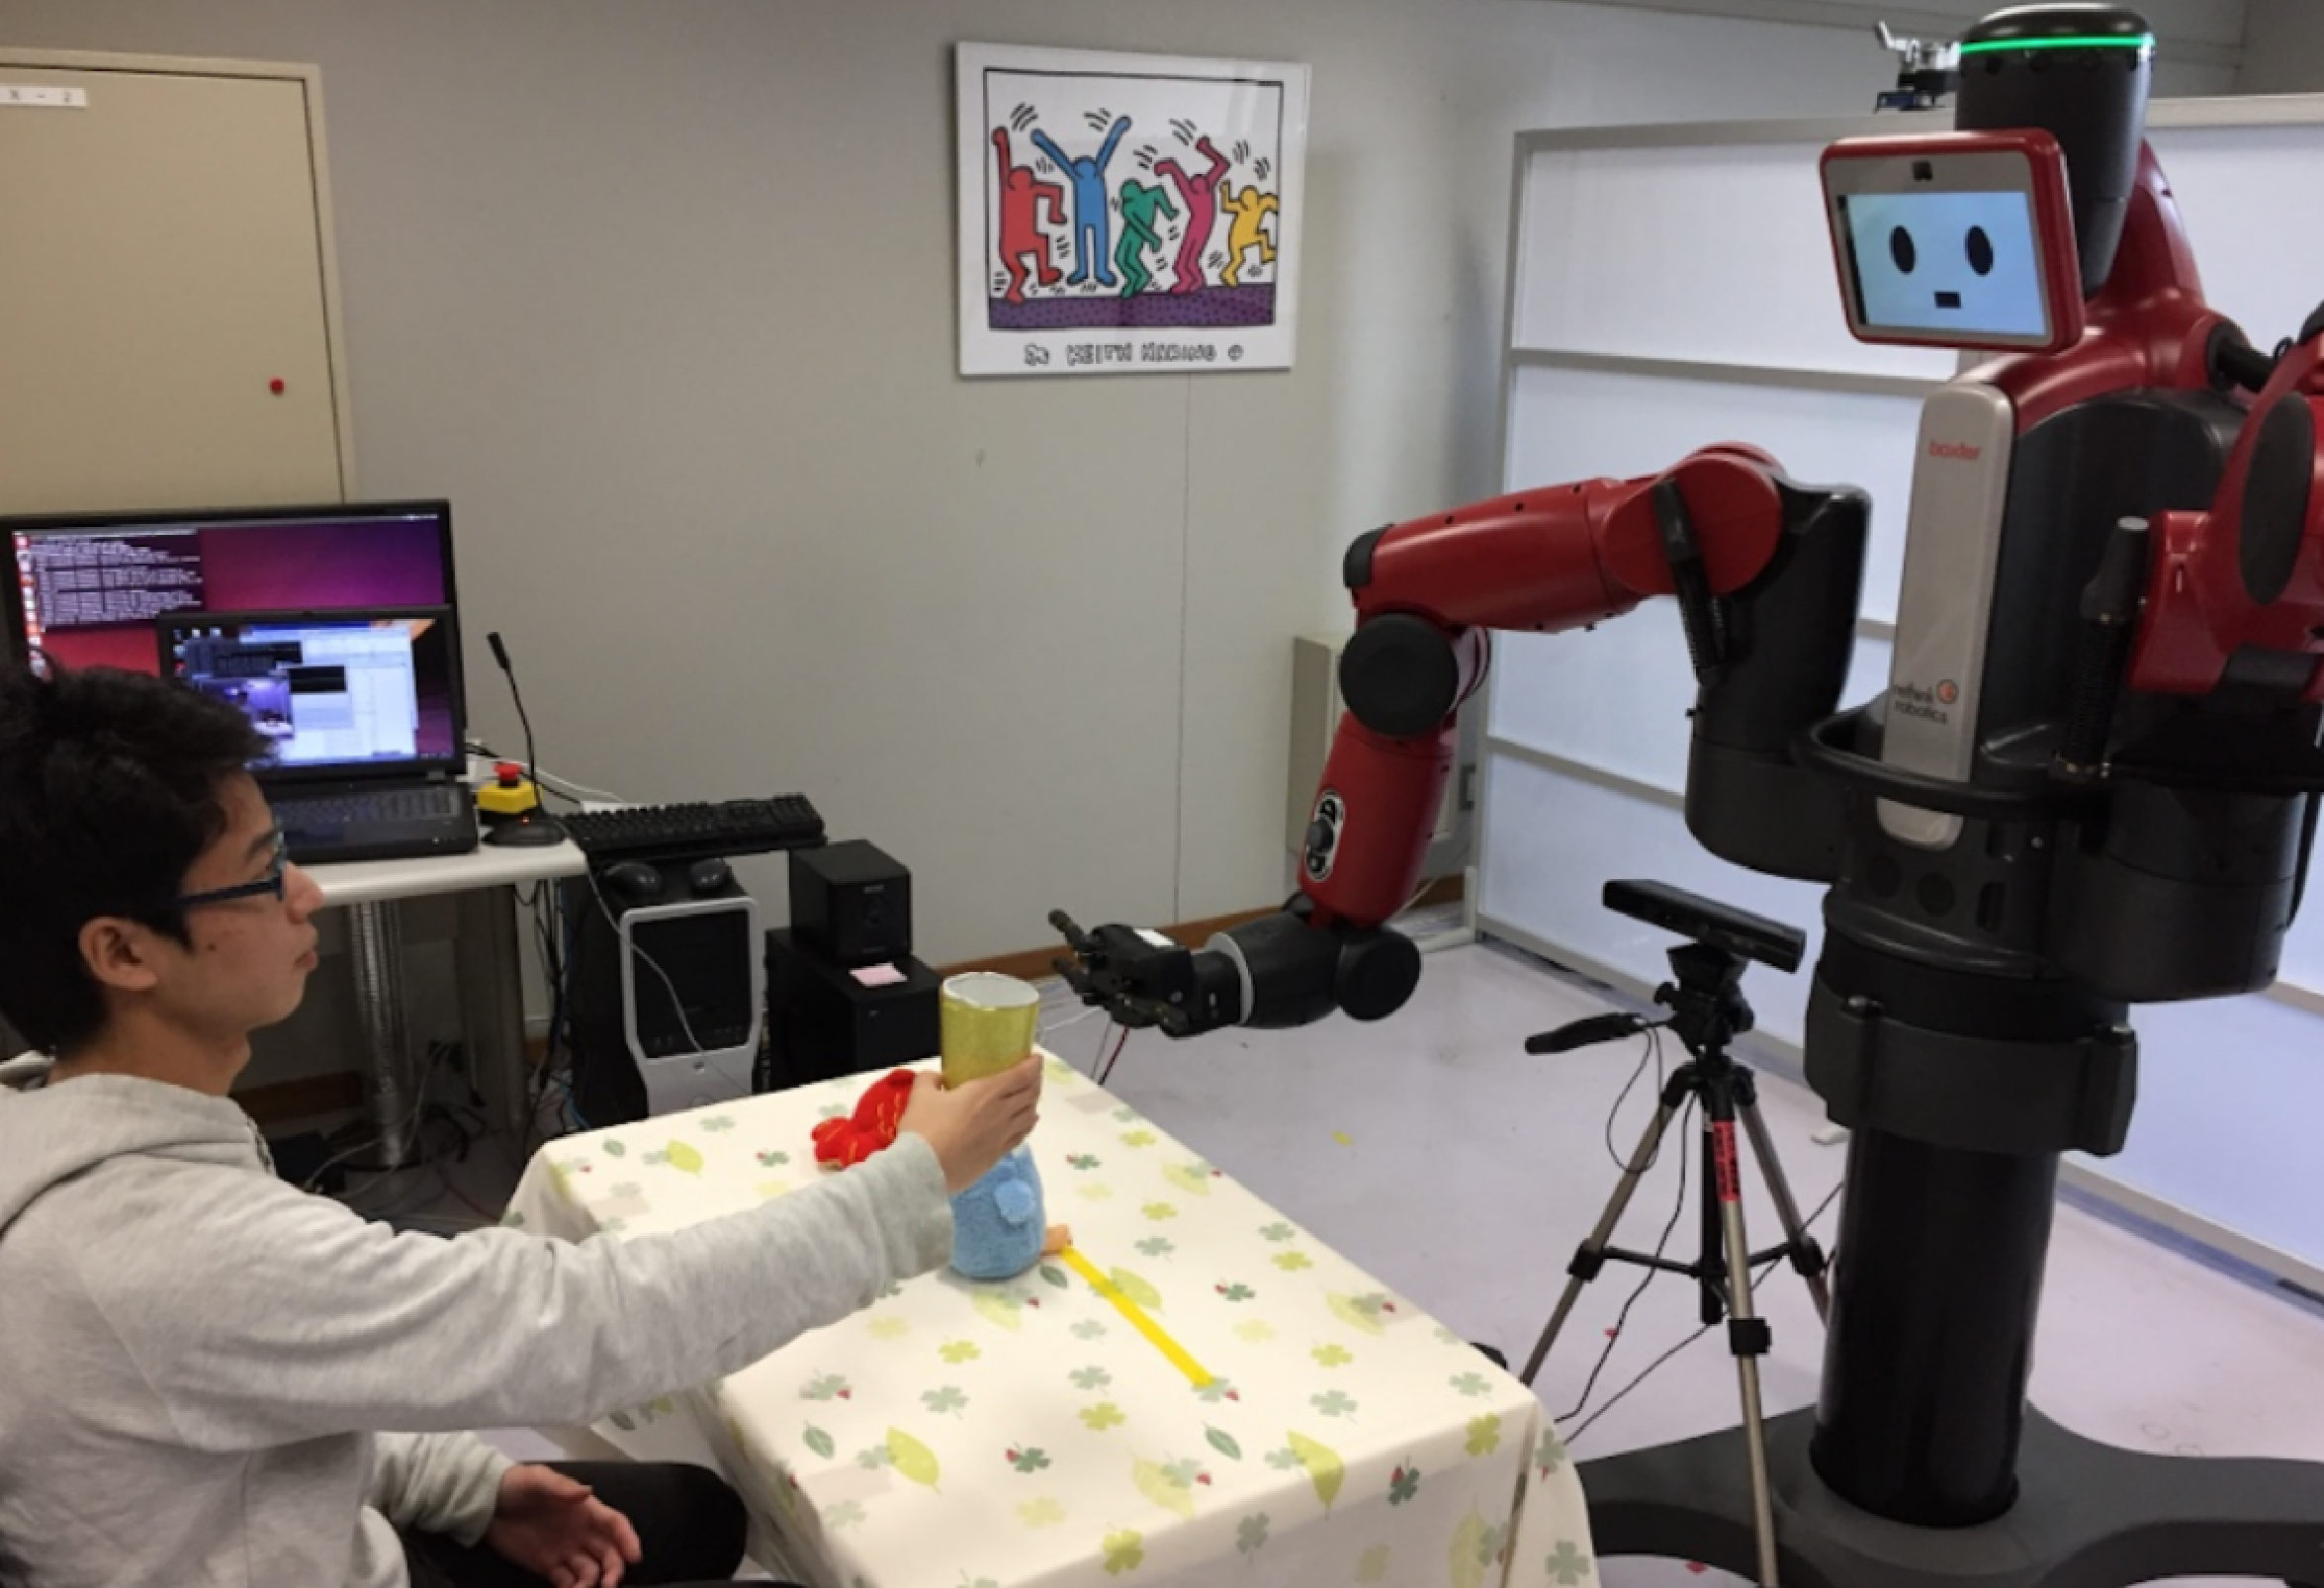
\includegraphics[width=0.9\columnwidth]{./fig/experimental_env.pdf}
      \end{center}
    \end{block}

    \begin{block}{3. Example Dialogue}
      \begin{itemize}
        \item Some examples of dialogue between human and robot:
      \end{itemize}

    \begin{table}
       %\caption{table caption}
        \label{tab:dialogue}
        \begin{tabular}{|l||l|}
        \hline
           Do you know any toys? & I am not familiar with toy.  \\
        \hline
           Here is the stuffed toy. & Oh, I see.  \\
        \hline
           Do you like animals? & I like dogs.  \\
        \hline
           I like this penguin. & I got it. \\
        \hline
        \end{tabular}
    \end{table}

    \end{block}
  \end{column} % End of the 1st column

%%%%%%%%%%%%%%%%%%%%%%%%%%%%%%%%%%%%%%%%%%
%% Column 2
%%%%%%%%%%%%%%%%%%%%%%%%%%%%%%%%%%%%%%%%%%

  \begin{column}{.02\textwidth}\end{column} % Empty spacer column

  \begin{column}{.3\textwidth} % 2nd column
    \vspace{\shrink}
    \begin{block}{4. Propose Method}
  %    \textbf{Method details.} We formulate... $\mathcal S = \{s_1, s_2, s_3, s_4, s_5, s_6 \}$
      \begin{center}
        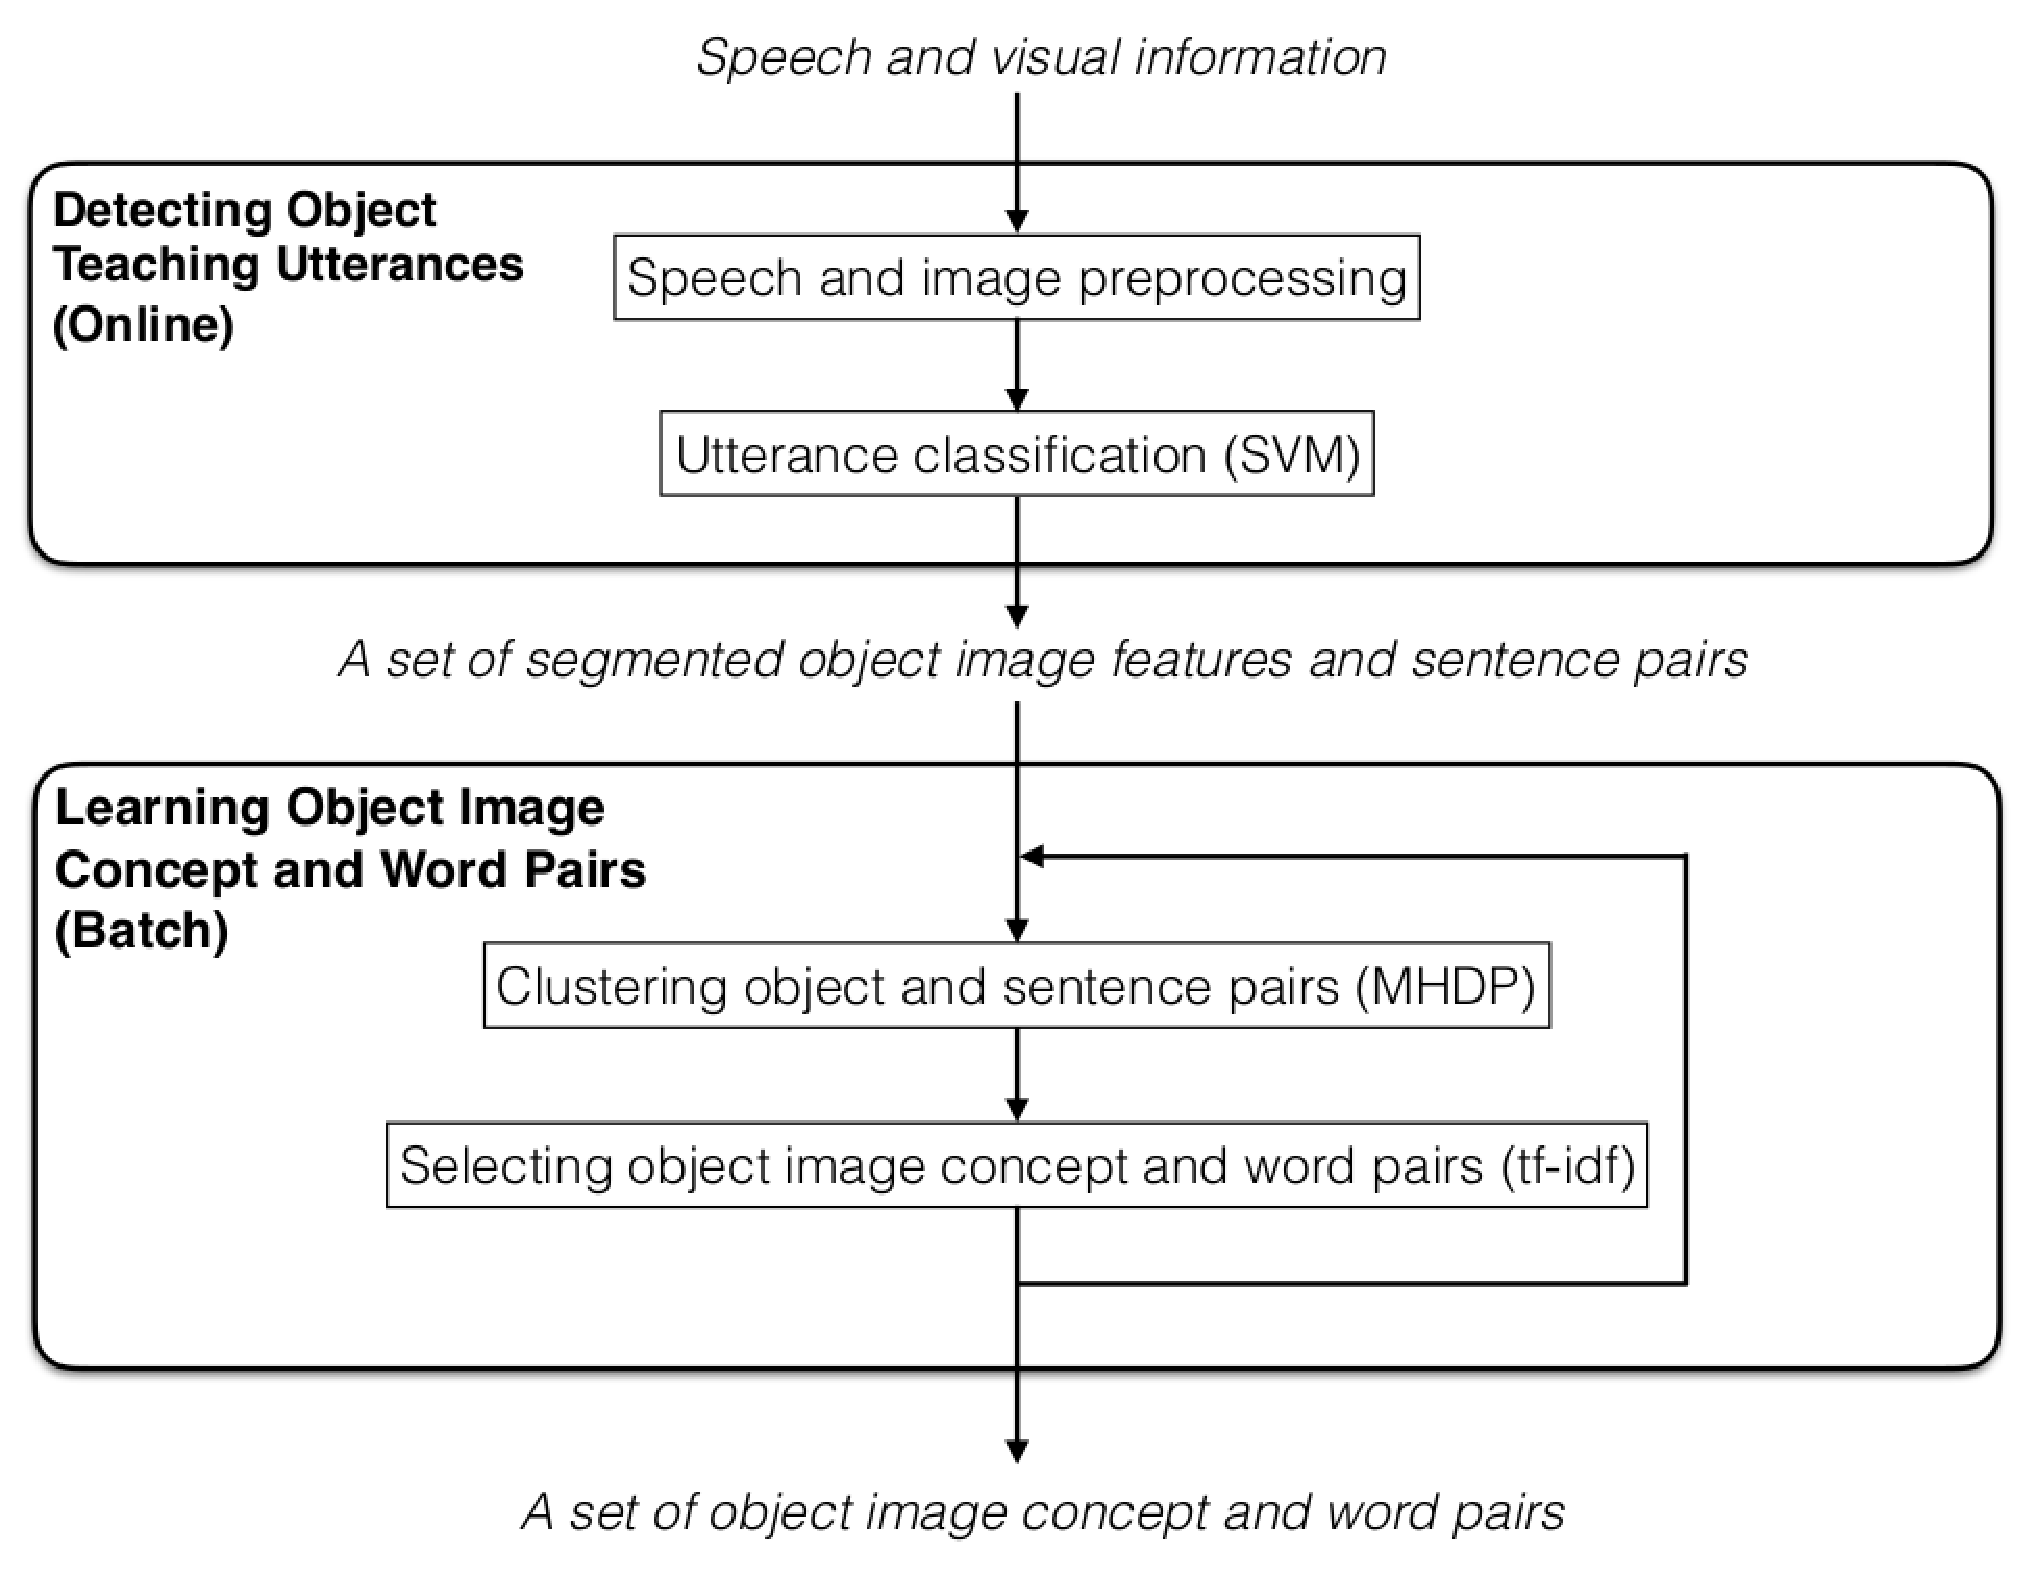
\includegraphics[width=0.9\columnwidth]{./fig/propose_method.pdf}
      \end{center}
    \end{block}

    \begin{block}{5. Learning Method (MHDP+tf-idf)}
      %Block text \cite{le-2016-inference-compilation}...
      \begin{center}
        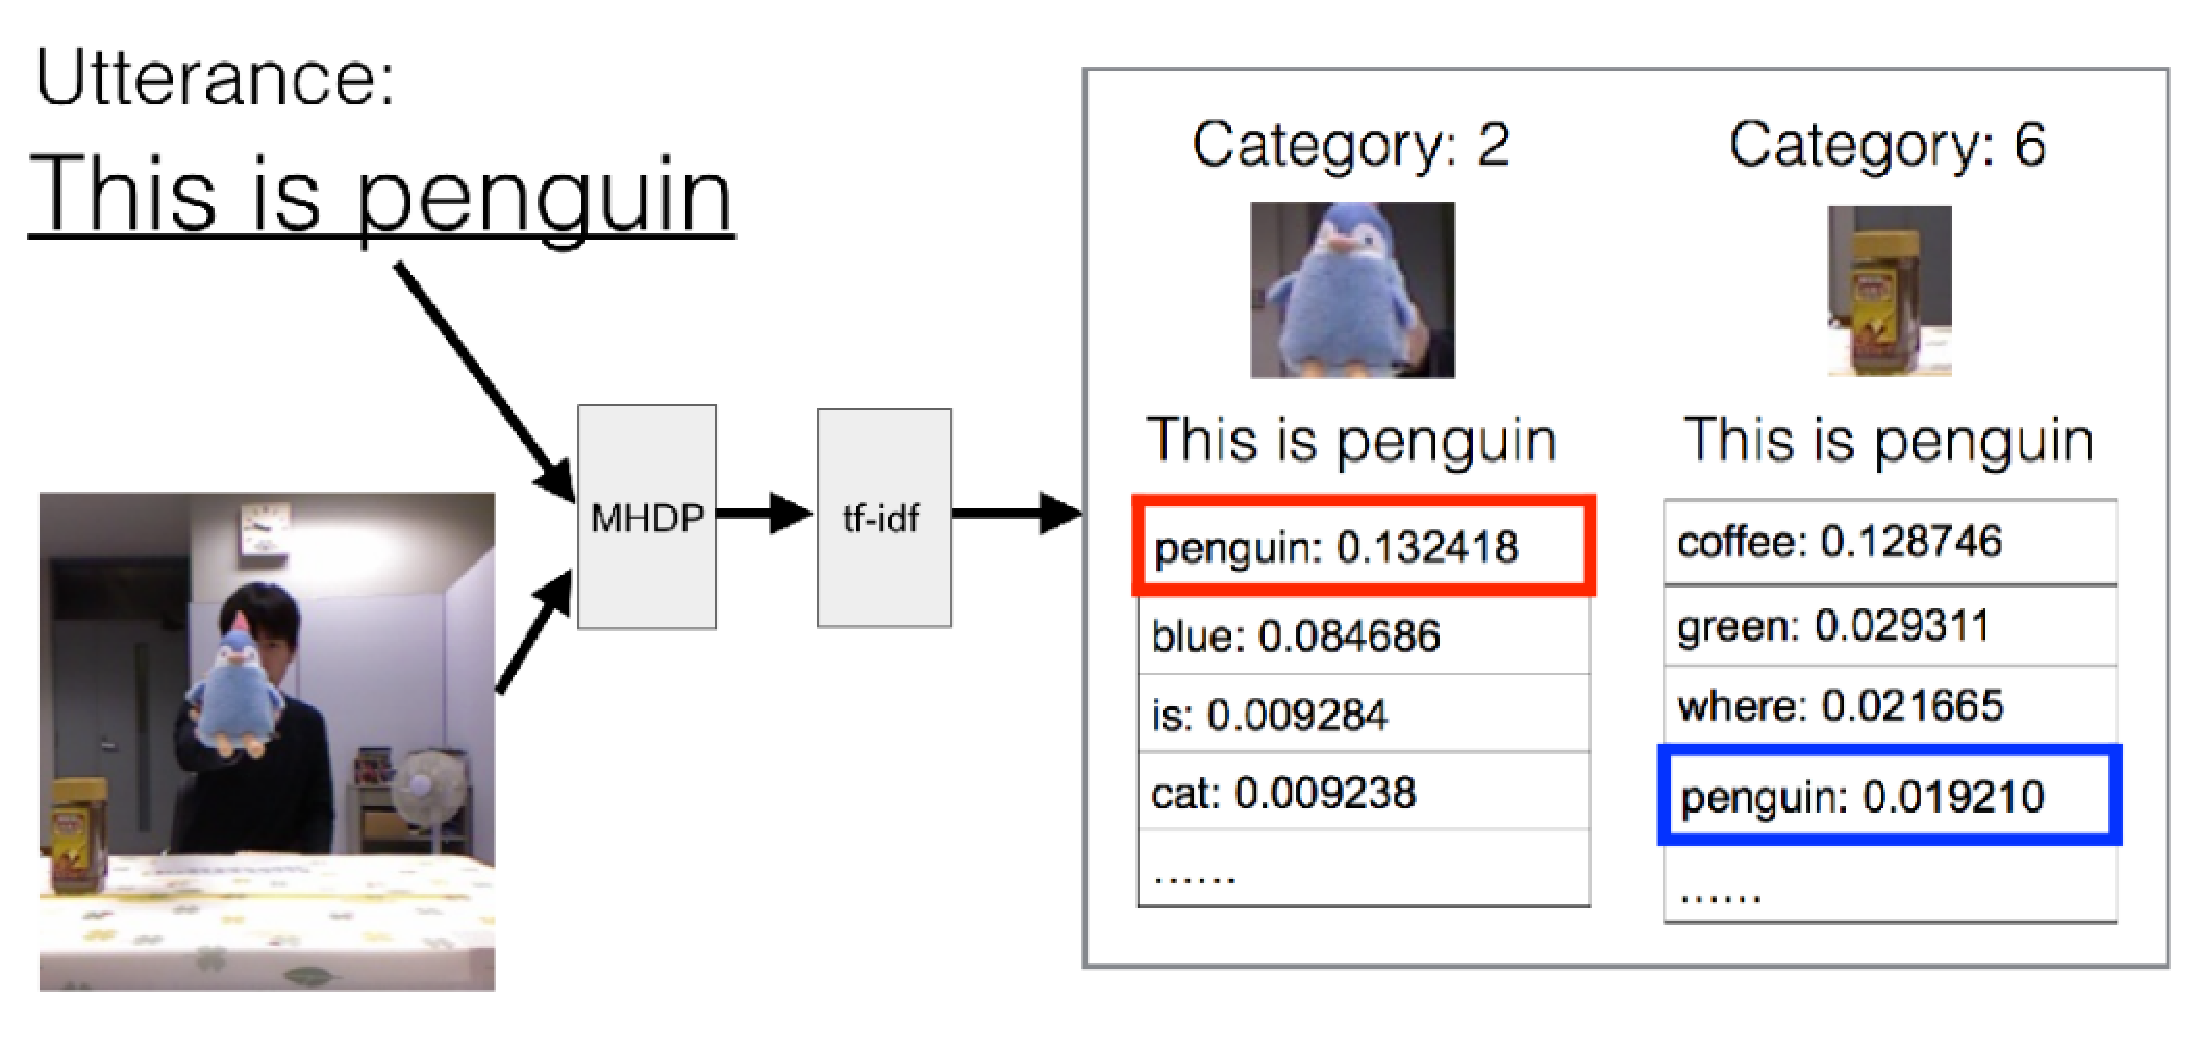
\includegraphics[width=0.9\columnwidth]{./fig/learning_method.pdf}
      \end{center}
    \end{block}

    \begin{block}{6. Experimental Setup}
The ten objects used in the experiment are: two black stuffed toy cats (small \& big), two stuffed toy fishes (red \& yellow), and two cups (red \& yellow)\\
      \begin{center}
        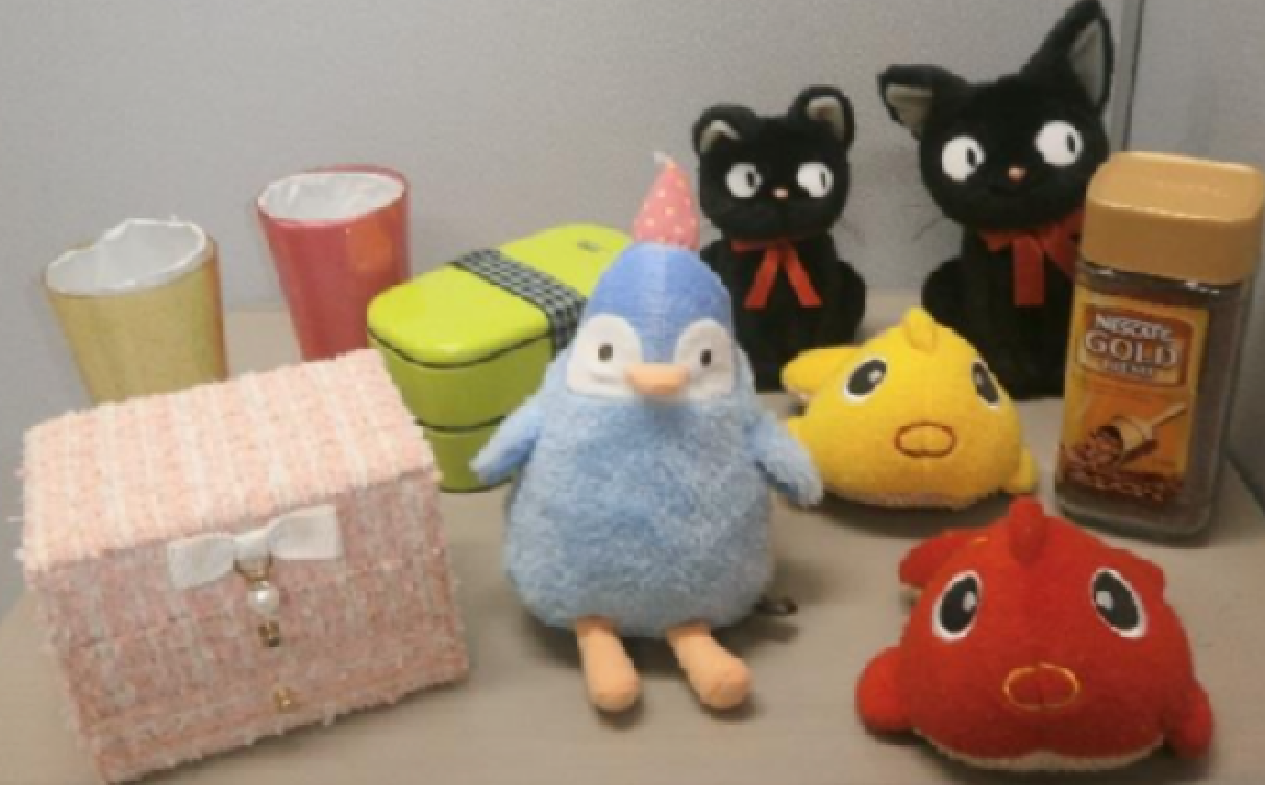
\includegraphics[width=0.4\columnwidth]{./fig/ten_objects.pdf}
      \end{center}
    \end{block}

  \end{column} % End of the 2nd column

%%%%%%%%%%%%%%%%%%%%%%%%%%%%%%%%%%%%%%%%%%
%% Column 3
%%%%%%%%%%%%%%%%%%%%%%%%%%%%%%%%%%%%%%%%%%

  \begin{column}{.02\textwidth}\end{column} % Empty spacer column

  \begin{column}{.3\textwidth} % 3rd column

    \begin{block}{7. Results}
      Results... \\
    \begin{table}
       \caption{Results of learning accuracy of object and words (\%)}
        \label{tab:result}
        \begin{tabular}{|c||c|c|c|}
        \hline
           without loop & 31\% (61/196) & 30\% (59/196) &  10\% (19/196) \\
        \hline
           with loop & 35\% (69/196) & 57\% (112/196) & 28\% (54/196) \\
        \hline
        \end{tabular}
    \end{table}
    Here, 
    \begin{itemize}
        \item $P_{w}$: probability of selecting correct word in each sentence
        \item $P_{c}$: probability of selecting object image concept for each sentence
        \item $P_{wc}$: probability of selecting both correct word and object image concept for each sentence
        \item Result: \textcolor{red}{without loop $<$ with loop}
    \end{itemize}
    \end{block}

    \begin{block}{References}
      \nocite{*} % Insert publications even if they are not cited in the poster
      \linespread{0.928}\selectfont
      \footnotesize{\bibliographystyle{unsrt}
      \bibliography{acet_poster}}
    \end{block}

    \begin{block}{Acknowledgments}
    \begin{itemize}
    \item This work was supported by JSPS KAKENHI (grant number 15K00244) and
JST CREST (“Symbol Emergence in Robotics for Future Human-Machine
Collaboration”)
    \end{itemize}
    \end{block}

  \end{column} % End of the 3rd column

  \begin{column}{.02\textwidth}\end{column} % Empty spacer column

\end{columns} % End of all the columns in the poster

\end{frame} % End of the enclosing frame

\end{document}
